
Im Folgenden sind die während des Versuchs aufgenommenen Messwerte sowie
die aus diesen berechneten Messergebnisse tabellarisch aufgeführt. An 
entsprechender Stelle sind Anmerkungen und Erklärungen zu den 
Rechnungen gegeben. Die jeweils mit aufgeführten Fehler der Ergebnisse 
wurden mit den mit römischen Zahlen nummerierten Gleichungen in \cref{sec:Fehlerrechnung}
berechnet, die jeweilige Gleichung ist dabei angegeben.

\subsection{Direkte Bestimmung der Ruhewellenlänge}
\label{sec:Auswertung_Wellenlänge}	
	Die Messwerte zur Bestimmung der Ruhewellenlänge, des verwendeten Signals 
	sind in \cref{tab:Auswertung_Wellenlänge} zusammen mit den daraus bestimmten Werten für die Wellenlänge
	und deren Inverses eingetragen.
	
	\begin{table}[!h]
	\centering
	\begin{tabular}{|c|c|c|c|}
		\hline
		Strecke & Wellenlängenanzahl & Wellenlänge & inverse Wellenlänge\\
		$s\,[\si{\meter}]$ & $n$ & $\lambda\,[\si{\meter}]$ & $\lambda^{-1}\,[\si{\per\meter}]$\\\hline\hline
		\num{0.0462(1)}  & \num{3.0}  & \num{0.01540(5)}  & \num{64.9(2)} \\
		\num{0.0465(1)}  & \num{2.5}  & \num{0.01860(6)}  & \num{53.8(2)} \\
		\num{0.0479(1)}  & \num{2.5}  & \num{0.01916(6)}  & \num{52.2(2)} \\
		\num{0.0493(1)}  & \num{2.5}  & \num{0.01972(6)}  & \num{50.7(1)} \\
		\num{0.0441(1)}  & \num{2.5}  & \num{0.01764(6)}  & \num{56.7(2)} \\
		\hline
	\end{tabular}
	\caption{Messdaten der Wellenlängenbestimmung und Wellenlänge sowie inverse Wellenlänge \label{tab:Auswertung_Wellenlänge}}
\end{table}   
	
	Für die zu untersuchende inverse Wellenlänge erhält man daraus den Mittelwert
	\begin{empheq}{equation}
		\label{eq:Auswertung_Wellenlaenge_direkt}
		\left<\lambda_{0}^{-1}\right> = \SI{56(2)}{\per\meter}.
	\end{empheq}
	Dabei ist der angegebene Fehler
	die Abweichung vom Mittelwert und nicht durch Fehlerfortpflanzung bestimmt, da
	diese Abweichungen wesentlich geringer ausfallen.
	 
\subsection{Bestimmung der Wagengeschwindigkeiten}

	Die zur Bestimmung der Wagengeschwindigkeiten in den verschiedenen Gängen
	aufgenommenen Fahrtdauern über die Messstrecke 
	\begin{empheq}{equation}
		\label{eq:Auswertung_Strecke}
		\left< l \right> = \SI{0.458(1)}{\meter}
	\end{empheq}
	sind in \cref{tab:Auswertung_Fahrtzeiten} angegeben.
	
	\begin{table}[!h]
	\centering
	\begin{tabular}{|c|c|c|c|c|}
		\hline
		Gang &  \multicolumn{2}{c|}{Zeit hin} & \multicolumn{2}{c|}{Zeit zurück}\\
		$g$ & $t_{h1}\,[\si{\second}]$ & $t_{h2}\,[\si{\second}]$ & $t_{r1}\,[\si{\second}]$ & $t_{r2}\,[\si{\second}]$\\\hline\hline
		\num{6}  & \num{9.10(1)}  & \num{9.09(1)}  & \num{9.05(1)}  & \num{9.03(1)} \\
		\num{12}  & \num{4.55(1)}  & \num{4.55(1)}  & \num{4.52(1)}  & \num{4.52(1)} \\
		\num{18}  & \num{3.03(1)}  & \num{3.04(1)}  & \num{3.01(1)}  & \num{3.02(1)} \\
		\num{24}  & \num{2.28(1)}  & \num{2.29(1)}  & \num{2.26(1)}  & \num{2.25(1)} \\
		\num{30}  & \num{1.82(1)}  & \num{1.82(1)}  & \num{1.81(1)}  & \num{1.83(1)} \\
		\num{36}  & \num{1.52(1)}  & \num{1.59(1)}  & \num{1.51(1)}  & \num{1.51(1)} \\
		\num{42}  & \num{1.30(1)}  & \num{1.31(1)}  & \num{1.34(1)}  & \num{1.30(1)} \\
		\num{48}  & \num{1.14(1)}  & \num{1.19(1)}  & \num{1.13(1)}  & \num{1.13(1)} \\
		\num{54}  & \num{1.02(1)}  & \num{1.02(1)}  & \num{1.00(1)}  & \num{1.00(1)} \\
		\num{60}  & \num{0.92(1)}  & \num{0.91(1)}  & \num{0.91(1)}  & \num{0.90(1)} \\
		\hline
	\end{tabular}
	\caption{Fahrtdauern des Wagens in den verschiedenen Gängen \label{tab:Auswertung_Fahrtzeiten}}
\end{table}
	
	Aus den hieraus, jeweils für Hin- und Rückfahrt, gemittelten Zeiten und der 
	Messstrecke \cref{eq:Auswertung_Strecke} lassen sich die Geschwindigkeiten 
	des Wagens für die unterschiedlichen Gänge in \cref{tab:Auswertung_Geschwindigkeiten} 
	berechnen.
	
	\begin{table}[!h]
	\centering
	\begin{tabular}{|c|c|c|}
		\hline
		Gang & Geschwindigkeit & Geschwindigkeit\\
		$g\,[\si{}]$ & $v_{h1}\,[\si{\meter\per\second}]$ & $v_{h2}\,[\si{\meter\per\second}]$\\\hline\hline
		\num{6.000}  & \num{0.05036(9)}  & \num{0.05066(9)} \\
		\num{12.000}  & \num{0.1007(2)}  & \num{0.1013(2)} \\
		\num{18.000}  & \num{0.1509(4)}  & \num{0.1519(4)} \\
		\num{24.000}  & \num{0.2004(7)}  & \num{0.2031(7)} \\
		\num{30.000}  & \num{0.252(1)}  & \num{0.252(1)} \\
		\num{36.000}  & \num{0.295(1)}  & \num{0.303(1)} \\
		\num{42.000}  & \num{0.351(2)}  & \num{0.347(2)} \\
		\num{48.000}  & \num{0.393(2)}  & \num{0.405(3)} \\
		\num{54.000}  & \num{0.449(3)}  & \num{0.458(3)} \\
		\num{60.000}  & \num{0.501(4)}  & \num{0.506(4)} \\
		\hline
	\end{tabular}
	\caption{Geschwindigkeiten des Wagens in den verschiedenen Gängen \label{tab:Auswertung_Geschwindigkeiten}}
\end{table} 
 	
 	
	
\subsection{Bestimmung von Ruhefrequenz und Schallgeschwindigkeit}
\label{sec:Auswertung_FrequenzSchall}
	Zur direkten Bestimmung der Frequenzänderung muss zunächst die Ruhefrequenz
	des verwendeten Signals bestimmt werden, die dafür genommenen Messwerte  
	sind in \cref{tab:Auswertung_Ruhefrequenz} zu finden.  
	
	\begin{table}[!h]
	\centering
	\begin{tabular}{|c||c|}
		\hline
		Ruhefrequenz & Ruhefrequenz\\
		$\nu_{0}\,[\si{\hertz}]$ & $\nu_{0}\,[\si{\hertz}]$\\\hline\hline
		\num{20165(1)} &\num{20166(1)} \\
		\num{20165(1)} &\num{20166(1)} \\
		\num{20166(1)} &\num{20166(1)} \\
		\num{20113(1)} &\num[color=red]{19915(1)} \\
		\num[color=red]{19646(1)} &\num[color=red]{19773(1)} \\
		
		
	
		
		
		
		
		\hline
	\end{tabular}
	\caption{Gemessene Ruhefrequenzen \label{tab:Auswertung_Ruhefrequenz}}
\end{table}	
	
	Für die Berechnung des Mittelwertes wurden die hervorgehobenen Werte nicht verwendet,
	da diese eine zu große Abweichung zu den übrigen Messwerten aufweisen. Es folgt
	der Mittelwert mit der Abweichung vom diesem
	\begin{empheq}{equation}
		\label{eq:Auswertung_Ruhefrequenz}
		\left< \nu_{0} \right> = \SI{20158(7)}{\hertz}.
	\end{empheq} 
	
	Aus dieser Ruhefrequenz $\left< \nu_{0} \right>$ und der zuvor bestimmten inversen Wellenlänge 
	\cref{eq:Auswertung_Wellenlaenge_direkt} kann nun die Schallgeschwindigkeit $c$ zu
	\begin{empheq}{equation}
		\label{eq:Auswertung_Schallgeschwindigkeit}
		c =\left<  \lambda_{0} \right> \cdot \left< \nu_{0} \right> = \SI{362(15)}{\meter\per\second} \footnotemark
	\end{empheq}
	berechnet werde. 
	\footnotetext{Fehler berechnet durch \cref{std:Schallgeschwinigkeit}.}
	
	Mit der berechneten Schallgeschwindigkeit $c$, der Maximalgeschwindigkeit des Wagens 
	$v_{max}$ aus \cref{tab:Auswertung_Geschwindigkeiten} und der Ruhefrequenz $\nu_{0}$ 
	\cref{eq:Auswertung_Ruhefrequenz} lässt sich nun der Unterschied der beiden Gleichungen 
	\cref{eq:Theorie_BewegterEmpfänger} und \cref{eq:Theorie_BewegterSender} berechnen,
	da aus der Taylorentwicklung der letzteren 
	\begin{empheq}{equation}
		\nu_{Q} = \nu_{E} + \nu_{0} \cdot \mathcal{O}\del{\del{\dfrac{v}{c}}^{2}}
	\end{empheq} 
	gilt.
	Der größte Term der dieser Restglieder hat mit den bestimmten Größen den Wert
		\begin{empheq}{equation}
		\nu_{0} \cdot \del{\dfrac{v}{c}}^{2} = \SI{0.039(3)}{\hertz}
		\end{empheq} 
	und ist damit um zwei Größenordnungen kleiner als der angenommene Fehler bei den Frequenzmessungen.
	Daher ist bei dem verwendetem Versuchsaufbau keine Unterscheidung zwischen bewegtem Sender und 
	Empfänger nötig beziehungsweise möglich.     
		
\subsection{Direkte Bestimmung der Frequenzänderung}
\label{sec:Auswertung_Direkt}
	Die für die verschiedenen Gänge gemessenen erhöhten beziehungsweise verringerten Frequenzen 
	während der Bewegung des Wagens sind in \cref{tab:Auswertung_Frequenz_Direkt} eingetragen.
	
	\begin{table}[!h]
	\centering
	\begin{tabular}{|c|c|c|c|c|}
		\hline
		Gang & Frequenz & Frequenz & Frequenz & Frequenz\\
		$g\,[\si{}]$ & $\nu_{h1}\,[\si{\hertz}]$ & $\nu_{h2}\,[\si{\hertz}]$ & $\nu_{r1}\,[\si{\hertz}]$ & $\nu_{r2}\,[\si{\hertz}]$\\\hline\hline
		\num{6.000}  & \num{20169(1)}  & \num{20168(1)}  & \num{20162(1)}  & \num{20163(1)} \\
		\num{12.000}  & \num{20171(1)}  & \num{20172(1)}  & \num{20160(1)}  & \num{20160(1)} \\
		\num{18.000}  & \num{20175(1)}  & \num{20175(1)}  & \num{20158(1)}  & \num{20157(1)} \\
		\num{24.000}  & \num{20178(1)}  & \num{20177(1)}  & \num{20154(1)}  & \num{20155(1)} \\
		\num{30.000}  & \num{20180(1)}  & \num{20180(1)}  & \num{20151(1)}  & \num{20151(1)} \\
		\num{36.000}  & \num{20183(1)}  & \num{20183(1)}  & \num{20148(1)}  & \num{20148(1)} \\
		\num{42.000}  & \num{20186(1)}  & \num{20186(1)}  & \num{20146(1)}  & \num{20145(1)} \\
		\num{48.000}  & \num{20189(1)}  & \num{20189(1)}  & \num{20143(1)}  & \num{20143(1)} \\
		\num{54.000}  & \num{20191(1)}  & \num{20192(1)}  & \num{20139(1)}  & \num{20139(1)} \\
		\num{60.000}  & \num{20195(1)}  & \num{20195(1)}  & \num{20137(1)}  & \num{20136(1)} \\
		\hline
	\end{tabular}
	\caption{Direkt gemessene Frequenzen des Wagens in den verschiedenen Gängen \label{tab:Auswertung_Frequenz_Direkt}}
\end{table}
	
	Aus den, aus diesen Messwerten, gemittelten Frequenzen für Hin- und Rückfahrt und der Ruhefrequenz
	\cref{eq:Auswertung_Ruhefrequenz} können nun die in \cref{tab:Auswertung_Frequenzänderung_Direkt} gelisteten 
	Frequenzdifferenzen für Hin- und Rückfahrt berechnet werden.
	
	\begin{table}[!h]
	\centering
	\begin{tabular}{|c|c|c|}
		\hline
		Gang & Differenzfrequenz & Differenzfrequenz\\
		$g\,[\si{}]$ & $\Delta \nu_{h}\,[\si{\hertz}]$ & $\Delta \nu_{r}\,[\si{\hertz}]$\\\hline\hline
		\num{6.000}  & \num{10(7)}  & \num{4(7)} \\
		\num{12.000}  & \num{13(7)}  & \num{2(7)} \\
		\num{18.000}  & \num{17(7)}  & \num{-1(7)} \\
		\num{24.000}  & \num{19(7)}  & \num{-4(7)} \\
		\num{30.000}  & \num{22(7)}  & \num{-7(7)} \\
		\num{36.000}  & \num{25(7)}  & \num{-10(7)} \\
		\num{42.000}  & \num{28(7)}  & \num{-13(7)} \\
		\num{48.000}  & \num{31(7)}  & \num{-15(7)} \\
		\num{54.000}  & \num{33(7)}  & \num{-19(7)} \\
		\num{60.000}  & \num{37(7)}  & \num{-22(7)} \\
		\hline
	\end{tabular}
	\caption{Frequenzänderungen des Wagens nach derDirekten Methode in den verschiedenen Gängen \label{tab:Auswertung_Frequenzänderung_Direkt}}
\end{table}  
	
	Diese Frequenzdifferenzen sind in \cref{fig:Auswertung_Frequenzänderung_direkt} grafische in Abhängigkeit von den 
	Geschwindigkeiten in \cref{tab:Auswertung_Geschwindigkeiten} dargestellt.
	Dabei sind die Geschwindigkeiten $ v_{h} $ auf das Mikrofon zu (hin) mit positivem Vorzeichen  
	und die $ v_{r} $ von diesem weg (zurück) mit negativem Vorzeichen versehen.
	
	\begin{figure}[!h]
		\centering
		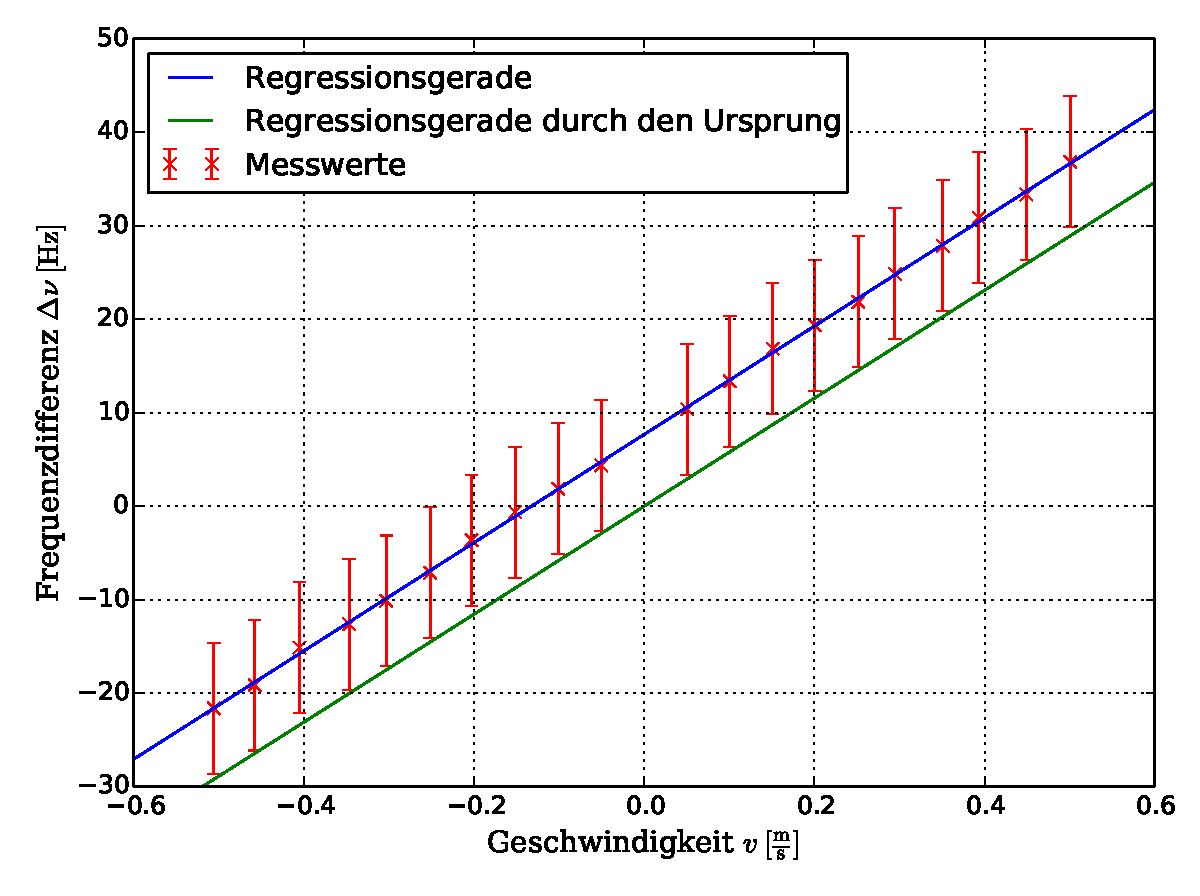
\includegraphics[scale=0.7]{Grafiken/Frequenzdifferenz_direkt.pdf}
		\label{fig:Auswertung_Frequenzänderung_direkt}
		\caption{Direkt bestimmte Frequenzänderung in Abhängigkeit der Geschwindigkeit\\\hspace*{2.6cm} mit entsprechenden Regressionsgeraden}
	\end{figure}  
	
	Die ebenfalls in \cref*{fig:Auswertung_Frequenzänderung_direkt} aufgetragene Regressionsgerade
	wurde mit Hilfe der Python-Bibliothek \emph{SciPy} \cite{SciPy} bestimmt. 
	Hierfür wurde ein Funktion der Form 
	\begin{empheq}{equation}
		g(v) =  A \cdot v + B
	\end{empheq}  
	als Ansatz gewählt.
	Die für diesen bestimmten Regressionsparameter $A\ \text{und}\ B$ ergeben sich durch die Regression
	zu
	\addtocounter{equation}{-1}
	\begin{subequations}
		\begin{empheq}{align}
				\label{eq:Auswertung_Paramter_A1}
				A &= \SI{57.9(2)}{\per\meter}\\ 
				\label{eq:Auswertung_Paramter_B1}
				B &= \SI{7.69(8)}{\hertz} 
			\end{empheq} 
	\end{subequations}
	
	Nach \cref{eq:Theorie_BewegterEmpfänger} müsste die eingezeichnete Gerade jedoch durch 
	den Ursprung gehen, mit dieser Prämisse erhält man die zweite ebenfalls in 
	\cref{fig:Auswertung_Frequenzänderung_direkt} eingezeichnete Gerade, deren Parameter
	\addtocounter{equation}{-1}
	\begin{subequations}
	\addtocounter{equation}{2}
		\begin{empheq}{align}
				\label{eq:Auswertung_Paramter_A2}
				A' &= \SI{58(6)}{\per\meter}\\ 
				\label{eq:Auswertung_Paramter_B2}
				B' &= \SI{0}{\hertz} 
			\end{empheq} 
	\end{subequations}  
	
	Im Vergleich mit \cref{eq:Theorie_BewegterEmpfänger} ist nun offensichtlich, dass
	der Regressionsparameter $ A $ der inversen Ruhewellenlänge entspricht.
	Aufgrund der geringen Abweichung der Steigung $ A' $ von $ A $, wird hier der
	Wert mit dem geringeren Fehler für den späteren Vergleich als inverse Wellenlänge     
	\begin{empheq}{equation}
		\label{eq:Auswertung_InverseWellenlänge_direkt}
		\lambda_{0,direkt} = A = \SI{57.9(2)}{\per\meter}
	\end{empheq}
	verwendet.
	
\subsection{Bestimmung der Frequenzänderung mit der Schwebungsmethode}
\label{sec:Auswertung_Schwebung}
 	Die Messwerte, die für die Frequenzänderung mit Hilfe der Schwebungsmethode aufgenommen wurden 
 	befinden sich in \cref{tab:Auswertung_Frequenz_Schwebung} in der auch die Mittelwerte dieser 
 	Messwerte angegeben sind.
 	
 	\begin{table}[!h]
	\centering
	\begin{tabular}{|c|c|c|c|c|c|c|}
		\hline
 		Gang & \multicolumn{3}{c|}{Frequenzdifferenz hin} & \multicolumn{3}{c|}{Frequenzdifferenz zurück} \\
		$g$ & $\Delta\nu_{h1}\,[\si{\hertz}]$ & $\Delta\nu_{h2}\,[\si{\hertz}]$ & $\left<\Delta\nu_{h}\right>\,[\si{\hertz}]$ & $\Delta\nu_{r1}\,[\si{\hertz}]$ & $\Delta\nu_{r2}\,[\si{\hertz}]$ & $\left<\Delta\nu_{r}\right>\,[\si{\hertz}]$\\\hline\hline
		\num{6}  & -  & -  & -  & -  & -  & - \\
		\num{12}  & \num{4(1)}  & \num{4(1)}  & \num{4.0(7)}  & \num{-11(1)}  & \num{-12(1)}  & \num{-11.5(7)} \\
		\num{18}  & \num{14(1)}  & \num{14(1)}  & \num{14.0(7)}  & \num{-18(1)}  & \num{-18(1)}  & \num{-18.0(7)} \\
		\num{24}  & \num{17(1)}  & \num{18(1)}  & \num{17.5(7)}  & \num{-24(1)}  & \num{-23(1)}  & \num{-23.5(7)} \\
		\num{30}  & \num{16(1)}  & \num{14(1)}  & \num{15.0(7)}  & \num{-28(1)}  & \num{-29(1)}  & \num{-28.5(7)} \\
		\num{36}  & \num{20(1)}  & \num{19(1)}  & \num{19.5(7)}  & \num{-34(1)}  & \num{-34(1)}  & \num{-34.0(7)} \\
		\num{42}  & \num{28(1)}  & \num{24(1)}  & \num{26.0(7)}  & \num{-34(1)}  & \num{-35(1)}  & \num{-34.5(7)} \\
		\num{48}  & \num{33(1)}  & \num{32(1)}  & \num{32.5(7)}  & \num{-34(1)}  & \num{-33(1)}  & \num{-33.5(7)} \\
		\num{54}  & \num{35(1)}  & \num{36(1)}  & \num{35.5(7)}  & \num{-30(1)}  & \num{-28(1)}  & \num{-29.0(7)} \\
		\num{60}  & \num{39(1)}  & \num{56(1)}  & \num{47.5(7)}  & \num{-27(1)}  & \num{-23(1)}  & \num{-25.0(7)} \\
		\hline
	\end{tabular}
	\caption{Direkt gemessene Frequenzen des Wagens in den verschiedenen Gängen \label{tab:Auswertung_Frequenz_Schwebung}}
\end{table}
 	
 	In \cref{fig:Auswertung_Frequenzaenderung_Schwebung} sind die Mittelwerte der 
 	Frequenzänderungen gegen die Geschwindigkeiten aus 
 	\cref{tab:Auswertung_Geschwindigkeiten} zusammen mit zwei Regressionsgeraden aufgetragen.
 	Dabei sind diese analog zu der in \cref{sec:Auswertung_Direkt} beschrieben Weise mit Hilfe
 	\emph{SciPy} bestimmt worden und die entsprechenden Parameter des Ansatzes
	\begin{empheq}{equation}
		g(v) =  C \cdot v + D
	\end{empheq} 
	sind
	\addtocounter{equation}{-1}
	\begin{subequations}
		\begin{empheq}{align}
				\label{eq:Auswertung_Paramter_C1}
				C &= \SI{80(5)}{\per\meter}\\ 
				\label{eq:Auswertung_Paramter_D1}
				D &= \SI{-1(2)}{\hertz}
			\end{empheq} 
	\end{subequations}
	beziehungsweise
	\addtocounter{equation}{-1}
	\begin{subequations}
		\addtocounter{equation}{2}
		\begin{empheq}{align}
				\label{eq:Auswertung_Paramter_C2}
				C' &= \SI{80(5)}{\per\meter}\\ 
				\label{eq:Auswertung_Paramter_D2}
				D' &= \SI{0}{\hertz}. 
			\end{empheq} 
	\end{subequations}
	
 	\begin{figure}[!h]
 	 			\centering
 	 			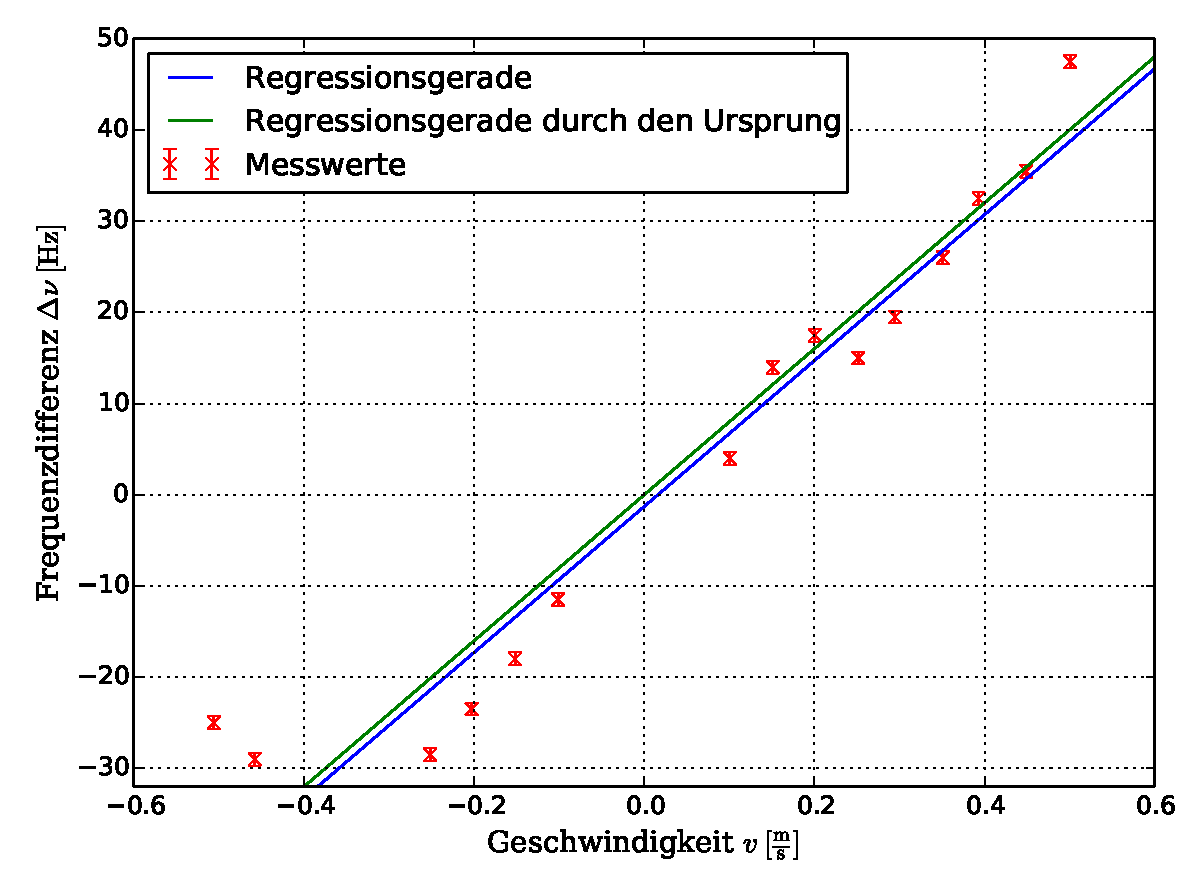
\includegraphics[scale=0.7]{Grafiken/Frequenzdifferenz_Schwebung.pdf}
 	 			
 	 			\caption{Mit der Schwebungsmethode bestimmte Frequenzänderung in Abhängigkeit der\\\hspace*{2.6cm} Geschwindigkeit mit entsprechenden Regressionsgeraden \label{fig:Auswertung_Frequenzaenderung_Schwebung}}
 	 		\end{figure} 
 	 		
 	Da auch diese Regressionsgerade die Form von \cref{eq:Theorie_BewegterEmpfänger} besitzt zeigt
 	sich, dass die Steigung der Geraden der inversen Ruhewellenlänge entspricht. 
	Da die beiden Geraden keinen Unterschied in ihrer Steigung aufweisen ergibt sich aus der Schwebungsmethode
	die inverse Wellenlänge
	\begin{empheq}{equation}
		\label{eq:Auswertung_InverseWellenlänge_Schwebung}
		\lambda_{0,Schwebung} = C = \SI{80(5)}{\per\meter}.
	\end{empheq}

\subsection{Beurteilung der Messergebnisse durch einen t-Test}
	
	Zur Beurteilung, ob zwischen zwei Messreihen $x_{i}$ und $y_{i}$ vom Umfang $n_{x}$ bzw. $n_{y}$ 
	der selben Messgröße ein systematischer Fehler besteht, kann der sogenannte studentsche t-Test verwendete werden.
	Für diesen benötigt man die Prüfgröße $t$ mit der Definition
	\begin{empheq}{equation}
		\label{eq:Auswertung_tTest_t}
		t = \dfrac{\mean{x} - \mean{y}}{\sigma_{\mean{x} - \mean{y}}}.
	\end{empheq} 	
	Die benötigten Größen sind dabei die Mittelwerte $\mean{x}$ und $\mean{y}$ der zwei zu vergleichenden Messreihen,
	sowie die Standardabweichung der Differenz dieser Mittelwerte $\sigma_{\mean{x} - \mean{y}}$, die unter der 
	Verwendung der Standardabweichungen der Mittelwerte $\sigma_{x}$ und $\sigma_{y}$ wie folgt definiert ist.
	\begin{empheq}{equation}
		\label{eq:Auswertung_tTest_s}
		\sigma_{\mean{x} - \mean{y}} = \sqrt{\dfrac{(n_{x} - 1)  \sigma_{x}^{2} + (n_{y} - 1)  \sigma_{y}^{2}}{(n_{x} - 1) + (n_{y} - 1)} \cdot 
		\dfrac{n_{x} + n_{y}}{n_{x}n_{y}}}
	\end{empheq} 
	In \cref{tab:Auswertung_StudentTest} sind die auf diese Weise berechneten Werte für  $\sigma_{\mean{x} - \mean{y}}$ und $t$ für die drei Vergleiche
	der Ergebnisse aus \cref{sec:Auswertung_Wellenlänge}, \ref{sec:Auswertung_Direkt} und \ref{sec:Auswertung_Schwebung} zu finden.
	Um eine Aussage über die Wahrscheinlichkeit eines systematischen Fehlers zwischen den Werten treffen zu können muss, ein aus der 
	Literatur \cite{Bortz10} entnommener Referenzwert $t_{ref}$ bekannt sein. Wird dieser von dem Betrag der Testgröße \envert{t} 
	überschritten so besteht mit der Wahrscheinlichkeit $1 - \alpha$ ein systematischer Fehler zwischen den Versuchsergebnissen.  
	Die Größe $\alpha$ ist damit die vor dem Test festzulegende Irrtumswahrscheinlichkeit, für diesen Test sei $\alpha = 0.01$. 	
	Die zu vergleichenden Werte seien hier noch einmal angegeben:
	\begin{empheq}{align*}
		\lambda_{0}   &= \SI{56(2)}{\per\meter} \\
		\lambda_{0,d} &=\SI{57.9(2)}{\per\meter}\\
		\lambda_{0,s} &=\SI{80(5)}{\per\meter}
	\end{empheq}
	
	
	\begin{table}[!h]
	\centering
	\begin{tabular}{|c|c|c|c|c|}
		\hline
		Vergleich & gewichtete Abweichung & Prüfgröße & Referenzwert & Wahrscheinlichkeit\\
		$ $ & $\sigma_{\mean{x} - \mean{y}}\,[\si{\per\meter}]$ & $\envert{t}$ & $t_{ref}$ & $P\,[\si{\percent}]$\\\hline\hline
		$\lambda_{0}\ \text{und}\ \lambda_{0,d}$  & \num{0.483}  & \num{4.668}  & \num{2.81}  & \num{99.0} \\
		$\lambda_{0}\ \text{und}\ \lambda_{0,S}$  & \num{2.219}  & \num{10.986}  & \num{2.81}  & \num{99.0} \\
		$\lambda_{0,S}\ \text{und}\ \lambda_{0,d}$  & \num{1.068}  & \num{20.707}  & \num{2.70}  & \num{99.0} \\
		\hline
	\end{tabular}
	\caption{Ergebnisse des Studentschen T-Tests \label{tab:Auswertung_StudentTest}}
\end{table}
	
	
	
	
	
	
	
	
	
	
	
	
	
	
	
	
	
	
	
	
	
	
	
	
	
	
	
	
	 